% Created 2011-05-23 Mon 11:41
\documentclass[11pt,english]{article}
\usepackage[utf8]{inputenc}
\usepackage[T1]{fontenc}
\usepackage{fixltx2e}
\usepackage{graphicx}
\usepackage{longtable}
\usepackage{float}
\usepackage{wrapfig}
\usepackage{soul}
\usepackage{textcomp}
\usepackage{marvosym}
\usepackage{wasysym}
\usepackage{latexsym}
\usepackage{amssymb}
\usepackage{hyperref}
\tolerance=1000

\usepackage{lmodern}
\renewcommand{\sfdefault}{lmss}
\renewcommand{\ttdefault}{lmtt}

% needed packages
\usepackage{amsmath}
\usepackage{amssymb}
\usepackage{amsthm}
\usepackage{babel}
\usepackage{epsfig}
\usepackage[T1]{fontenc}
\usepackage{fixltx2e}
\usepackage{float}
%\usepackage{floatflt}
\usepackage{graphics}
\usepackage{graphicx}
\usepackage[utf8]{inputenc}
\usepackage{latexsym}
\usepackage{longtable}
\usepackage{makeidx}
\usepackage{marvosym}
\usepackage{multicol}
%\usepackage{pslatex}
\usepackage{rotating}
%\usepackage{showidx}
\usepackage{soul}
\usepackage{srcltx}
\usepackage{stmaryrd}
\usepackage{subfig}
\usepackage{textcomp}
%\usepackage{theorem}
%\usepackage[subfigure]{tocloft}
\usepackage{txfonts}
\usepackage{upgreek}
\usepackage{url}
\usepackage{varioref}
%\usepackage{wasysym}
\usepackage{wrapfig}


% Page setup
\usepackage[paperwidth=8.5in,paperheight=11in]{geometry}
\geometry{verbose,tmargin=0.5in,bmargin=0.5in,lmargin=1in,rmargin=1in}




% PDF settings
%\usepackage[hyperref,x11names]{xcolor}
\usepackage{hyperref}
\hypersetup{pdftitle={STAT 5840: Statistical Computing},
 		pdfauthor={G. Jay Kerns}, 
		linkcolor=Firebrick4, 
		citecolor=black, 
		urlcolor=SteelBlue4}

% Listings setup
%\usepackage{color}
%\usepackage{listings}
%\lstset{basicstyle={\ttfamily},
%	language=R,
%	breaklines=true,
%	breakatwhitespace=true,
%	keywordstyle={\ttfamily},
%	numberstyle = {\ttfamily},
%	morestring=[b]"
%}



%  user defined commands
% special operators
\renewcommand{\P}{\mathrm{I\hspace{-1.5pt}P}}
\newcommand{\E}{\mathrm{I\hspace{-1.5pt}E}}
\renewcommand{\vec}[1]{\mbox{\boldmath$#1$}}

% special symbols
\newcommand{\me}{\mathrm{e}}
\newcommand{\R}{\mathbb{R}}
\newcommand{\diff}{\mathrm{d}}
\newcommand{\ybar}{\overline{y}}
\newcommand{\xbar}{\overline{x}}
\newcommand{\Xbar}{\overline{X}}
\newcommand{\Ybar}{\overline{Y}}





\providecommand{\alert}[1]{\textbf{#1}}

\title{Simulations with the Inversion/Transformation Methods}
%\author{G. Jay Kerns}
\date{STAT 5840: Summer 2011}

\begin{document}

\maketitle

\thispagestyle{empty}

\section*{Examples for Beta, Logistic, and Exponential}
\label{sec-1}


\begin{verbatim}
# SimTransMeth.R

par(mfrow = c(3,1))
Iter <- 10000                        # initialization and storage    
y <- rep(0, times = Iter)

# To simulate Beta(3,7)'s 
for (i in seq.int(Iter)){            # start the simulation loop        
  u <- sum(-log(runif(3)))           # a Gamma(a,1)
  v <- sum(-log(runif(7)))           # a Gamma(b,1)
  y[i] <- u/(u+v)                    # a Beta(a,b)
}
hist(y, 30, prob = TRUE, main = "Beta(3,7)")

# now plot the density function
f <- function(x) dbeta(x, shape1 = 3, shape2 = 7)
curve(f, lwd = 2, add = TRUE)


# To simulate Logis(3,7)'s
u <- runif(Iter)                     # 10,000 uniforms
x <- log(u/(1-u))                    # std logistics
y <- 3 + 7*x                         # Logis(3,7)'s
hist(y, 30, prob = TRUE, main = "Logis(3,7)")

# now plot the density function
f <- function(x) dlogis(x, location = 3, scale = 7)
curve(f, lwd = 2, add = TRUE)


# To simulate Exp(3)'s
u <- runif(Iter)             # bunch of uniforms
y <- -3*log(1-u)             # bunch of exponentials
hist(y, 30, prob = TRUE, main = "Exp(3)")

# now plot the density function
f <- function(x) dexp(x, rate = 1/3)
curve(f, lwd = 2, add = TRUE)

par(mfrow = c(1,1))
\end{verbatim}

\begin{figure}[h!]
\centering
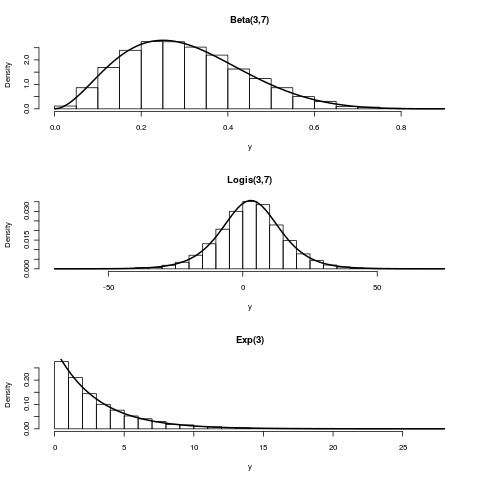
\includegraphics[width=7in, height=7in,]{img/SimTransInvMeth.pdf}
\caption{\label{fig:yplot}Plots of theoretical target densities, plus histograms of simulated values}
\end{figure}

\end{document}